\documentclass[tikz,border=5pt]{standalone}

\usepackage{fontspec}
\usepackage{unicode-math}
\usepackage{pgfplots}
\usepgfplotslibrary{groupplots}

\pgfplotsset{compat=1.18}

% Compile with LuaLaTeX or XeLaTeX.
\setmainfont{STIX Two Text}
\setmathfont{STIX Two Math}

\colorlet{functioncolor}{red!75!black}
\colorlet{midpointcolor}{blue!65!black}
\colorlet{gausscolor}{orange!85!black}

\begin{document}

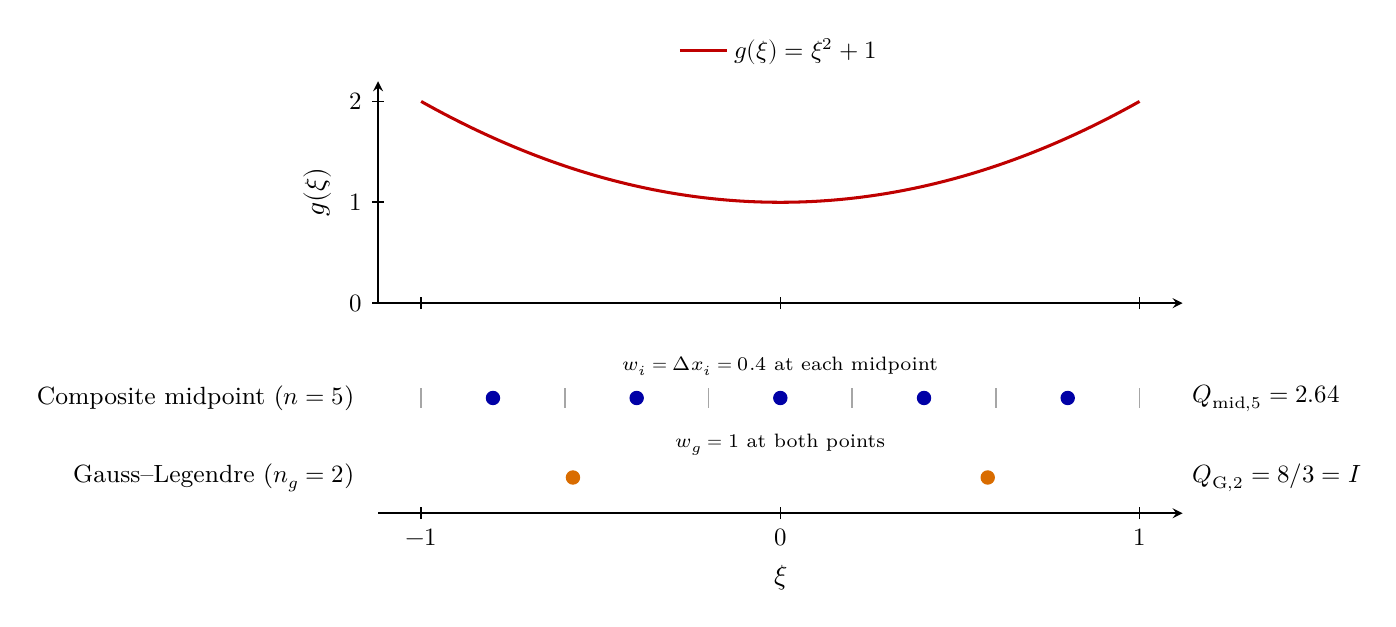
\begin{tikzpicture}

  \begin{groupplot}[
      group style={
          group size=1 by 2,
          vertical sep=0.75cm,
        },
      width=11.8cm,
      xmin=-1.12, xmax=1.12,
      axis line style={black, semithick},
      tick style={black, semithick},
      tick align=outside,
      tick label style={font=\small},
      label style={font=\normalsize},
      clip=false,
    ]

    % Integrand on the reference interval.
    \nextgroupplot[
      height=4.4cm,
      ymin=0, ymax=2.2,
      ylabel={\(g(\xi)\)},
      xtick={-1,0,1},
      xticklabels=\empty,
      ytick={0,1,2},
      axis lines=left,
      axis on top,
      legend style={
          at={(0.5,1.03)},
          anchor=south,
          draw=none,
          fill=none,
          font=\small,
        },
    ]

    \addplot[
      domain=-1:1,
      samples=150,
      functioncolor,
      line width=1.1pt,
    ] {x^2+1};
    \addlegendentry{\(g(\xi)=\xi^2+1\)}

    % Evaluation points and results.
    \nextgroupplot[
      height=3.5cm,
      ymin=-0.45, ymax=1.45,
      xlabel={\(\xi\)},
      xtick={-1,0,1},
      ytick=\empty,
      axis x line=bottom,
      axis y line=none,
      ytick style={draw=none},
    ]

    \node[anchor=east, xshift=-5pt, font=\small] at (axis cs:-1.12,1)
    {Composite midpoint (\(n=5\))};
    \node[anchor=east, xshift=-5pt, font=\small] at (axis cs:-1.12,0)
    {Gauss--Legendre (\(n_g=2\))};

    % Five equal subintervals for the composite midpoint rule.
    \pgfplotsinvokeforeach{-1,-0.6,-0.2,0.2,0.6,1}{
      \draw[gray!70, semithick] (axis cs:#1,0.88) -- (axis cs:#1,1.12);
    }
    \addplot[
      only marks,
      midpointcolor,
      mark=*,
      mark size=2.4pt,
      forget plot,
    ] coordinates {(-0.8,1) (-0.4,1) (0,1) (0.4,1) (0.8,1)};
    \node[anchor=south, font=\scriptsize] at (axis cs:0,1.16)
    {$w_i=\Delta x_i=0.4$ at each midpoint};
    \node[anchor=west, font=\small] at (axis cs:1.12,1)
    {\(Q_{\mathrm{mid},5}=2.64\)};

    % The two Gauss points.
    \addplot[
      only marks,
      gausscolor,
      mark=*,
      mark size=2.4pt,
      forget plot,
    ] coordinates {({-1/sqrt(3)},0) ({1/sqrt(3)},0)};
    \node[anchor=south, font=\scriptsize] at (axis cs:0,0.16)
    {\(w_g=1\) at both points};
    \node[anchor=west, font=\small] at (axis cs:1.12,0)
    {\(Q_{\mathrm{G},2}=8/3=I\)};

  \end{groupplot}

\end{tikzpicture}

\end{document}
